%% This is file `prletters-template.tex',
%% 
%% Copyright 2013 Elsevier Ltd
%% 
%% This file is part of the 'Elsarticle Bundle'.
%% ---------------------------------------------
%% 
%% It may be distributed under the conditions of the LaTeX Project Public
%% License, either version 1.2 of this license or (at your option) any
%% later version.  The latest version of this license is in
%%    http://www.latex-project.org/lppl.txt
%% and version 1.2 or later is part of all distributions of LaTeX
%% version 1999/12/01 or later.
%% 
%% The list of all files belonging to the 'Elsarticle Bundle' is
%% given in the file `manifest.txt'.
%% 
%% Template article for Elsevier's document class `elsarticle'
%% with harvard style bibliographic references
%%
%% $Id: prletters-template-with-authorship.tex 69 2013-07-15 10:15:25Z rishi $
%%
%% This template has no review option
%% 
%% Use the options `twocolumn,final' to obtain the final layout
\documentclass[times,twocolumn,final,authoryear]{elsarticle}

%% Stylefile to load PR Letters template
\usepackage{prletters}
\usepackage{framed,multirow}

%% The amssymb package provides various useful mathematical symbols
\usepackage{amssymb}
\usepackage{latexsym}

% Following three lines are needed for this document.
% If you are not loading colors or url, then these are
% not required.
\usepackage{url}
\usepackage{xcolor}
\definecolor{newcolor}{rgb}{.8,.349,.1}


\journal{Pattern Recognition Letters}

\begin{document}

\thispagestyle{empty}
                                                             
\begin{table*}[!th]

\begin{minipage}{.9\textwidth}
\baselineskip12pt
\ifpreprint
  \vspace*{1pc}
\else
  \vspace*{-6pc}
\fi

\noindent {\LARGE\itshape Pattern Recognition Letters}
\vskip6pt

\noindent {\Large\bfseries Authorship Confirmation}

\vskip1pc


{\bf Please save a copy of this file, complete and upload as the 
``Confirmation of Authorship'' file.}

\vskip1pc

As corresponding author 
I, Pablo Rozas Larraondo, 
hereby confirm on behalf of all authors that:

\vskip1pc

\begin{enumerate}
\itemsep=3pt
\item This manuscript, or a large part of it, \underline {has not been
published,  was not, and is not being submitted to} any other journal. 

\item If \underline {presented} at or \underline {submitted} to or
\underline  {published }at a conference(s), the conference(s) is (are)
identified and  substantial \underline {justification for
re-publication} is presented  below. A \underline {copy of
conference paper(s) }is(are) uploaded with the  manuscript.

\item If the manuscript appears as a preprint anywhere on the web, e.g.
arXiv,  etc., it is identified below. The \underline {preprint should
include a  statement that the paper is under consideration at Pattern
Recognition  Letters}.

\item All text and graphics, except for those marked with sources, are
\underline  {original works} of the authors, and all necessary
permissions for  publication were secured prior to submission of the
manuscript.

\item All authors each made a significant contribution to the research
reported  and have \underline {read} and \underline {approved} the
submitted  manuscript. 
\end{enumerate}

Signature\underline{\hphantom{\hspace*{7cm}}} Date\underline{\hphantom{\hspace*{4cm}}} 
\vskip1pc

\rule{\textwidth}{2pt}
\vskip1pc

{\bf List any pre-prints:}
\vskip5pc


\rule{\textwidth}{2pt}
\vskip1pc

{\bf Relevant Conference publication(s) (submitted, accepted, or
published):}
\vskip5pc



{\bf Justification for re-publication:}

\end{minipage}
\end{table*}

\clearpage
\thispagestyle{empty}
\ifpreprint
  \vspace*{-1pc}
\fi

\begin{table*}[!th]
\ifpreprint\else\vspace*{-5pc}\fi

\section*{Graphical Abstract (Optional)}
To create your abstract, please type over the instructions in the
template box below.  Fonts or abstract dimensions should not be changed
or altered. 

\vskip1pc
\fbox{
\begin{tabular}{p{.4\textwidth}p{.5\textwidth}}
\bf Type the title of your article here  \\
Author's names here \\[1pc]

\includegraphics[width=.3\textwidth]{top-elslogo-fm1.pdf}

Comparison of two different methods of splitting the space defined by a circular input variable in a regression tree.

%}\\
\end{tabular}
}

\end{table*}

\clearpage
\thispagestyle{empty}

\ifpreprint
  \vspace*{-1pc}
\else
%  \vspace*{-6pc}
\fi

\begin{table*}[!t]
\ifpreprint\else\vspace*{-15pc}\fi

\section*{Research Highlights (Required)}

To create your highlights, please type the highlights against each
\verb+\item+ command. 

\vskip1pc

\fboxsep=6pt
\fbox{
\begin{minipage}{.95\textwidth}
It should be short collection of bullet points that convey the core
findings of the article. It should  include 3 to 5 bullet points
(maximum 85 characters, including spaces, per bullet point.)  
\vskip1pc
\begin{itemize}

 \item

 \item A new method is presented to introduce circular variables inside regression trees.
 
 \item The proposed algorithm can combine linear and circular variables in the same tree.

 \item The proposed methodology reduces the computational cost of the algorithm from $\mathcal{O}(n^2)$ to $\mathcal{O}(n)$.

 \item This methodology outperforms previous proposals in both accuracy and computational cost.

\end{itemize}
\vskip1pc
\end{minipage}
}

\end{table*}

\clearpage


\ifpreprint
  \setcounter{page}{1}
\else
  \setcounter{page}{1}
\fi

\begin{frontmatter}

\title{Circular regression trees revisited}

\author[1]{Pablo \snm{Rozas Larraondo}\corref{cor1}}
\cortext[cor1]{Corresponding author:
  Tel.: +61-0414090095;}
\ead{pablo.larraondo@anu.edu.au}
\author[2]{I\~naki \snm{Inza}}
\author[2,3]{Jose A. \snm{Lozano}}

\address[1]{National Computational Infrastructure, Building 143, Australian National University, Ward Road, ACT, 2601, Australia}
\address[2]{Intelligent Systems Group, Computer Science Faculty, University of the Basque Country, Paseo de Manuel Lardizabal, Donostia, 20018, Spain}
\address[3]{Basque Center for Applied Mathematics (BCAM), Mazarredo 14, Bilbao, 48009, Spain}



\received{1 May 2013}
\finalform{10 May 2013}
\accepted{13 May 2013}
\availableonline{15 May 2013}
\communicated{S. Sarkar}


\begin{abstract}
Regression trees are a popular machine-learning method for making predictions using continuous variables. Circular variables have been used in regression trees by considering them as linear variables. A methodology to generate regression trees that understands circular variables was introduced by Lund in 2006. Lund's method recursively splits a circular space generating non-contiguous regions, requiring a $\mathcal{O}(n^2)$ computational cost. In this paper we introduce a new methodology for incorporating circular variables into regression trees where the computational cost is reduced to $\mathcal{O}(n)$. A series of experiments demonstrates this gain in computational performance and accuracy when compared to other methodologies. This methodology is especially suitable for training trees or ensembles of trees using large data sets that include circular variables.
\end{abstract}

\begin{keyword}
\MSC 41A05\sep 41A10\sep 65D05\sep 65D17
\KWD circular statistics\sep regression trees\sep time series\sep machine learning

%% MSC codes here, in the form: \MSC code \sep code
%% or \MSC[2008] code \sep code (2000 is the default)
\end{keyword}

\end{frontmatter}

%\linenumbers

%% main text
\section{Introduction}
\label{intro}
Circular data are prevalent in many scientific domains, such as earth sciences, ecology or medicine. Circular data are present in any directional measurement or variable with an inherent periodicity. Wind direction, angles in molecules or time stamped data containing times of day are examples of circular data.

Most of the current regression machine learning algorithms are focused on modelling the relationships between linear variables. Circular variables have a different nature to linear variables, so traditional methods cannot be applied or lead to wrong results in most of the cases.

A decision tree is a predictive model in which a data set is recursively partitioned based on values of the input variables, leading to smaller partitions used to estimate the target variable. A binary tree is a tree data structure in which each node has either two children or none. Classification and Regression Trees (CART) \citep{Breimanetal1984} is one of the most popular versions of binary decision trees to perform regressions. Lund \citep{Lund2002}, introduces a methodology that demonstrates how circular variables can be incorporated to regression trees. The concept of circular regression trees substantially differs from the CART model, introducing a higher complexity and computational cost to be trained. 

Regression trees have been a popular and effective technique in forecasting linear variables. Their simplicity and fast training characteristics make them a perfect candidate to be used with ensemble techniques, where a large number of trees are trained sampling the initial data set in different ways.

As the size of scientific data sets rapidly grows, there is an urgent need to come up with efficient algorithms that are able to cope with this growth. This paper proposes a different methodology to incorporate circular variables into regression trees, reducing the computational cost from $\mathcal{O}(n^2)$ to $\mathcal{O}(n)$. This methodology is similar to the one defined by CART, which has the benefit that it is very simple and easy to produce algorithms that implement it.

The sections in this paper are structured in the following way: Section 2 covers the basics of circular variables and how basic statistics are calculated. Section 3 contains a detailed description of different ways of creating regression trees, first for linear variables and second for circular variables. The section ends with a theoretical comparison between the original and proposed methodology for building circular regression trees. Section 4 contains a series of experiments that compare efficiency and accuracy figures for classic linear regression trees and both versions of circular regression trees. Section 5 contains the conclusions and proposes some lines that could be further investigated based on this work.

\section{Circular statistics}
A circular variable is defined as a numerical variable whose values are constrained into a cyclical space. For example, a variable measuring angles in radians, spans between 0 and 2$ \pi $, where both values represent the same point in space.

Circular statistics is the field of statistics that studies circular variables. Due to the different nature of circular variables, basic statistics, such as the mean or standard deviation, need to be calculated using different methods than the ones used for linear variables. A sample mean of a linear variable is normally calculated using the arithmetic mean of the observations. The arithmetic mean cannot be used to estimate the mean of a circular variable. For example, if the arithmetic mean formula is used to estimate the mean of the arc degrees with values 1 and 359, the result is (1 + 359)/2 = 180, which is different to the expected 0 or 360.

Fisher \citep{Fisher1992} presents the definition of vector $ \vec{\rho} $, which provides a convenient way of characterising circular variables. Considering a list of values$ [\alpha_1, \alpha_2, \dots, \alpha_n] $ representing a sample of a circular variable with values comprising $ [0, 2\pi] $, the vector $ \vec{\rho} $ is defined as:

\begin{displaymath}
\vec{\rho} = \left(\frac{1}{n}\cdot\sum_{i=1}^n \sin\alpha_i, \frac{1}{n}\cdot\sum_{i=1}^n \cos\alpha_i\right)
\end{displaymath}

This formula aggregates the contribution of all the different values in the sample into one vector. The argument of $ \vec{\rho} $ represents the mean and its module can be related to the variance of the sample. The estimators for the mean $ \hat{\theta}_{\mu} $ and for the standard deviation $ \hat{\theta}_{\sigma} $ are defined as: 

$ \hat{\theta}_{\mu} $ and $ \hat{\theta}_{\sigma} $ represent the mean and standard deviation of the sample, respectively. $ \hat{\theta}_{\sigma} $ is a function with range [0, 1] where 0 indicates that all the values are equal and 1 indicates maximum dispersion in the sample.


\section{Circular Regression Trees}

Circular Regression Trees is a concept proposed by Lund \citep{Lund2002} to introduce circular covariates in regression trees. Lund, in his paper, builds upon Breiman's earlier work on Classification and Regression Trees (CART) \citep{Breimanetal1984}. Lund discusses the particularities of circular variables and designs a methodology to create regression trees that can combine categorical, linear and circular variables.

Lund bases his argument on the lack of meaning that '$<$' and '$>$' operators have, when applied to a circular space. These operators, used on a circular variable, only define a sense of traversing a cyclic space but the definition of a value inside the circular space does not split it in two halves. Lund proposes instead to define regions and use the '$\in$' and '$\notin$' operators to create a recursive partitioning of a circular space. 

This approach succeeds in incorporating circular variables to regression trees, but it introduces a high level of complexity to the tree. In the following sections these complexities will be discussed and a new way of building regression trees combining linear and circular variables will be proposed. The next subsection explores the differences and effects that the use of these two sets of operators have on classic linear regression trees. Later, the concept of circular regression tree is introduced. It presents Lund's proposal and compares it with the proposed new methodology to build circular regression trees. The third and last subsection discusses the differences between Lund's and our methodology, comparing their efficiency and the accuracy of the results.

\subsection{Building Linear Regression Trees}

Regression trees, as presented by Breiman \citep{Breimanetal1984}, are built from a learning sample of observations. Let us consider a sample of observations $\mathcal{L}$ of linear variables $ x_1, x_2, \dots, x_n $ as a set of vectors $\bf{x} $ $= (x_1, x_2, \dots, x_n)$. In regression, a case consists of data $(\bf{x},$ $y)$ where $\bf{x}$ denotes measurement vectors, and $ y $ refers to the response or dependent variable. The measurement space $\mathcal{X}$ contains all possible measurement vectors. Each measurement vector in the observations sample can be represented as a point in the defined measurement space of dimension $n$. Different methods of regression analysis provide different functions $d(\bf{x})$, to estimate a value of the response variable $y$.

CART defines a way of selecting the best binary split at each non-terminal node, as well as a $d(\bf{x})$ function that provides the output at terminal nodes of a tree. These splits recursively divide the measurement space $\mathcal{X}$ in two parts. Using the '$<$' and '$>$' operators, $\mathcal{X}$ is divided along the axis of one of the covariates $x_i$ each time.

Figure \ref{f1} contains a reproduction of the example used by Breiman to represent the partition of the measurement space $\mathcal{X}$ performed by a regression tree.

% For two-column wide figures use
\begin{figure*}
% Use the relevant command to insert your figure file.
% For example, with the graphicx package use
  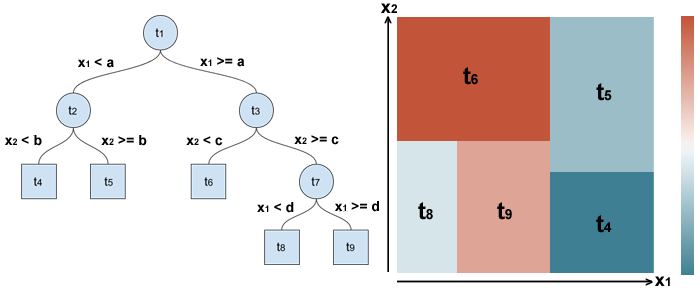
\includegraphics[width=17cm]{fig1_master.png}
% figure caption is below the figure
\caption{Example of a classic linear regression tree and a representation of how the space is divided. }
\label{f1}       % Give a unique label
\end{figure*}
%
 
As can be seen in Figure \ref{f1}, nodes $t1$ and $t7$ of the sample tree select values along the $x_1$ axis, to split the space in two halves. Similarly, $t2$ and $t3$ select values along the $x_2$ axis to divide the space.

Linear regression trees recursively partition the space, finding the best split at each non-terminal node, by identifying a value of one of its covariates. The measurement space $\mathcal{X}$ will be divided in two halves by that value, along the axis of the selected covariate. To determine the best split at a node, CART only needs to identify one value for one of the covariates.

Although CART provides a methodology to easily divide the measurement space at the nodes of a tree, this is not the only way of doing it. The use of different operators, such as those proposed by Lund ('$\in$' and '$\notin$'), will result in a different partition of the space. The $in$ '$\in$' and $not in$ '$\notin$' notation comes from the set theory. Its use can be extended to denote that a value belongs or not to a determined range within a linear space. Using a similar sample of observations to the previous example, Figure \ref{f2} shows an example of how the measurement space is divided using the new operators.

%
% For two-column wide figures use
\begin{figure*}
% Use the relevant command to insert your figure file.
% For example, with the graphicx package use
  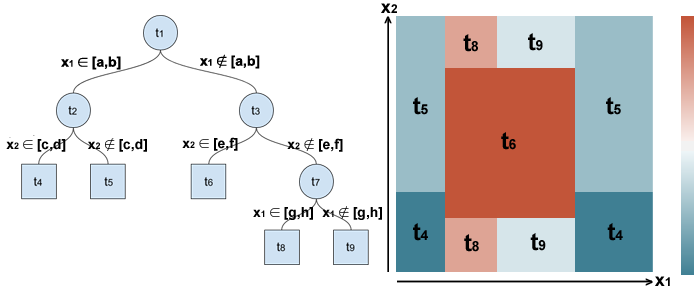
\includegraphics[width=17cm]{fig2_master.png}
% figure caption is below the figure
\caption{Example of a linear regression tree that uses the '$\in$' and '$\notin$' operators and a representation of how the space is divided.}
\label{f2}       % Give a unique label
\end{figure*}
%

The most noticeable difference between the last two figures is that the resulting regions defined by the tree are spatially contiguous in Figure 1 whereas some of the regions corresponding same nodes of the tree appear as non-contiguous in Figure \ref{f2}. This new way of dividing the space requires finding a range of values within the covariate’s space. The split is determined by the values that belong and do not belong to that range. Finding a range instead of a value is also a perfectly valid proposal, but has computational implications, which will be discussed in Section 3.3, and depending of the data set, it can also have a negative impact on the accuracy of the resulting tree.

\textbf{\textit{Non-contiguous splits generate partitions in which distant parts of a data set are aggregated into the same node. For example, Figure \ref{f2} displays data corresponding to node $t_5$ split at both ends of axis $x_1$. Intuitively, data inside these two separated regions might not be as correlated as the data delimited by a single contiguous region. As a consequence, nodes containing non-contiguous splits might degenerate in accuracy for successive partitions when compared to contiguous splits.}}


\subsection{Building Circular Regression Trees}

This section considers how circular variables can be assimilated by regression trees. A circular space is cyclic, it does not have bounds and even the notion of a minimum and maximum values does not apply. The distance between two values in the space is also an ambiguous concept, as it can be measured in clockwise and anticlockwise directions yielding different results. For these reasons the '$<$' and '$>$' operators are ill defined in circular spaces.

Lund's proposition to introduce ranges, solves the problem of univocally defining a region within a circular space. If $\alpha$ is a circular variable defined in $[0, 2\pi]$, a range within that variable can be determined by $arc(\alpha_1, \alpha_2)$. The '$\in$' and '$\notin$' operators are used to designate two regions of the circular space that belong and do not belong to that range, respectively. These two regions represent two complementary and non-overlapping regions in the circular space.

To illustrate how a circular tree partitions the space, a similar example to the one shown in the previous subsection is used. In this case, the tree contains one linear variable $x$ and one circular variable $\alpha$. Instead of using a Cartesian reference system to represent the partitions, a polar coordinate system is used to represent the circular nature of $\alpha$. In an analogous way to how splits for linear trees where presented, Figure \ref{f3} depicts the partitions performed by a sample circular tree.

%
% For two-column wide figures use
\begin{figure*}
% Use the relevant command to insert your figure file.
% For example, with the graphicx package use
  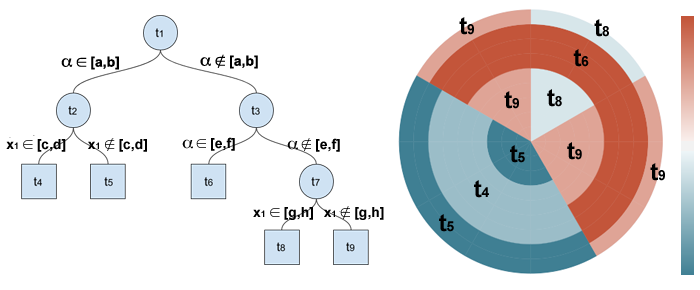
\includegraphics[width=17cm]{fig3_master.png}
% figure caption is below the figure
\caption{Example of a circular regression tree as formulated by Lund and a representation of how the space is divided.}
\label{f3}       % Give a unique label
\end{figure*}
%


Figure \ref{f3} shows an example of how a circular tree partitions the space defined by one linear and one circular variables. In a similar way as was shown by Figure \ref{f2}, the space is divided in non-contiguous regions along both its axes. \textbf{\textit{In this example, node $t_9$ contains data corresponding to four different regions of the space, which might limit the possibilities of finding subsequent good splits.}}  

It is worth noting that the previous example does not exactly represent a circular tree as introduced by Lund. What Lund proposes is the use of the '$\in$' and '$\notin$' operators just for the circular variables and the '$>$' and '$<$' operators for the linear ones. Therefore, circular trees produce non-contiguous regions only when a node of the tree creates a split based on a circular variable.

The space splitting performed by the '$>$' and '$<$' operators in classical trees can be seen as a particular case of the more general range selection performed by the '$\in$' and '$\notin$' operators in circular trees. The former assumes the bounds of the space to remain constant and finds a value within its range to split it in two contiguous regions. The latter, on the other hand, finds an inner sub-region contained in a space by identifying two delimiter values. These two values also define an outer sub-region, one at each side of the inner one, which is therefore non-contiguous.

The process described in Section 3.1, based on the '$>$' and '$<$' operators, can be seen as a particular case of the more general search in the space performed by the '$\in$' and '$\notin$' operators. Any contiguous split can be seen as a subset in which one of its bounds is shared with the original space. Partitioning the space by using the '$\in$' and '$\notin$' operators generates all the contiguous and non contiguous splits. As it considers more options, it will have better chances of finding a good partition, at the expense of doing more computations. The next subsection provides a quantitative comparison between the computational cost of building trees using contiguous and non-contiguous splits.

It is worth noting that for any circular variable, two values have to be provided in order to define two separate regions. In the case of a circular variable in a tree, its first split divides the circular space in two complementary arcs. Once these limits have been defined, values within an arc can be sorted by defining one direction (clockwise or counterclockwise) of traversing the space. Having a sortable space means that the '$>$' and '$<$' operators acquire meaning, and splits can be generated by selecting just one value within an arc.

Non-contiguous spaces appear in circular trees as a consequence of using the same '$\in$' and '$\notin$' operators for subsequent splits of a circular variable. As pointed out in the previous paragraph, after the first split of a circular variable, once regions have been defined, the splitting method used by classic regression trees can be used to generate contiguous partitioned spaces. This is the essential difference between our proposal and Lund's version of circular regression trees and is the main contribution of this work.

Figure \ref{f4} provides a graphical representation of our proposed methodology that generates contiguous circular trees applied to the same example data set. The benefits of generating contiguous splits in regression trees are discussed in the next section, considering differences in the computation efficiency and accuracy of their results.

%
% For two-column wide figures use
\begin{figure*}
% Use the relevant command to insert your figure file.
% For example, with the graphicx package use
  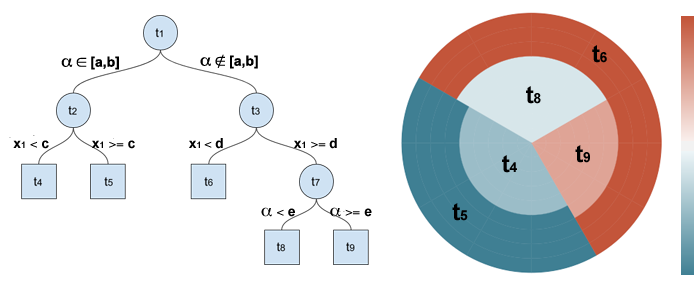
\includegraphics[width=17cm]{fig4_master.png}
% figure caption is below the figure
\caption{Example of the proposed circular regression tree and a representation of how the space is divided.}
\label{f4}       % Give a unique label
\end{figure*}
%


\subsection{Comparison between contiguous and non-contiguous splits: performance and accuracy.}

Regression trees are a very popular machine learning algorithm, because they are easy to use, they can represent non-linearities on the data and are relatively fast to train when compared to other methods such as support vector machines or neural networks. These characteristics make them a perfect candidate for ensemble methods such as bagging or boosting, where training hundreds or thousands of trees is needed. Ensemble methods using trees have demonstrated excellent results in many different fields and providing real time and streaming versions of them has been an active research field recently \citep{Abdulsalametal2007}.

Efficiency and computational cost of the different implementations of regression trees is relevant when the objective is to scale to a large number of trees. Optimising resources when analysing big data sets is of high interest nowadays, in order to reduce costs and execution times. There are several approaches for training trees using data sets that do not fit in the system memory \citep{Rokach2016}, such as SPRINT \citep{Shareretal1996}, SLIQ \citep{Mehtaetal1996} or FastC4.5 \citep{Heetal2007}. Most of the current efficient tree implementations are built upon the principles presented by these algorithms.

The building process of a regression tree can be separated in two phases: growth and prune. In the growth phase, the space is recursively partitioned, defining the nodes of the tree until the stop criteria is satisfied. The cost of evaluating splits in classic linear regression trees is dominated by the computational cost of sorting its values \citep{Shareretal1996}. All the possible splits are considered and evaluated, using a cost function to identify the best split. This operation has a computational cost of $\mathcal{O}(n)$, where $n$ represents the number of distinct elements contained by the variable.

Classic regression trees use a methodology which divides the space in two halves each time, by selecting one value within the range of its variables. The case of dividing the space in two halves by selecting one value is different to the case of having to find a subset contained anywhere within the range. This requires traversing the space considering all the possible combinations of the start and end bounds for the subset. This operation is much more expensive and has a quadratic complexity $\mathcal{O}(n^2)$.

Just the difference in the computational cost of these two splitting methods justifies the approach followed by classic regression trees when efficiency matters. In the next section, some experiments are carried out to compare the accuracy of both methodologies.

As has been demonstrated in the previous subsection, finding inner regions by defining both values for its boundaries, leads the tree to recursively fragment the space in non-contiguous or disjoint regions. Figure 5 shows an example where the space defined by a variable is recursively split, in a tree generating non-contiguous regions.

%
% For two-column wide figures use
% \begin{figure*}
% Use the relevant command to insert your figure file.
% For example, with the graphicx package use
%  \includegraphics[width=1.0\textwidth]{image002.png}
% figure caption is below the figure
% \caption{Example of recursive space fragmentation as a result of the use of non-contiguous splits.}
% \label{fig:5}       % Give a unique label
% \end{figure*}
%

Characterising the number of non-contiguous regions at each node is not an intuitive task. It depends on the number of nodes inherited from its parent node and on how the new split is made. This number is bounded by 1 and $l$, where $l$ represents the depth level of the node in the tree, starting at its root.

A consequence of this is that for deep trees, trees with a large number of levels, the fragmentation level at some of the nodes can be substantial. This contrasts with the case of classical regression tress, where each node contains just one contiguous region of the original data set at any level of the tree. Fragmentation of the space contained by nodes comes at the price of increasing the computational cost, memory consumption and complexity of the algorithm that generates the tree.

Efficient implementations of classical regression trees optimise memory consumption by storing references to regions of the original data set at each node. This model has the benefit that only one copy of the data set is stored in memory. If the data set is stored in the form of pre-sorted columns, each node will only have to keep two references: the minimum and maximum values of the variable, as proposed in SPRINT \cite{Shareretal1996}.

Fragmentation of the space forces the tree structure to keep track of the boundaries for each region. This increases the complexity of nodes and increments memory use proportionally to the number of fragments in the node. Many research efforts have been made in the field of disjoint set unions, and there are many strategies than can help to structure and optimise its performance \cite{RefI}. Nonetheless, working with contiguous regions makes unnecessary any optimisation of the algorithms and provides a simpler solution.

Table \ref{t1} represents a comparison between the number of non-contiguous regions stored by a particular node for different levels of a tree, considering contiguous and non-contiguous regions.

% For tables use
\begin{table*}[t]
\caption{Comparison of the growing complexity of tree nodes.}\label{t1}
\begin{center}
\begin{tabular}{rrrr}
\hline\hline
$Tree\ Level$ & $Max\ regions\ (Contiguous)$ & $Max\ regions\ (Non-Contiguous)$\\
\hline
$1$ & $0$ & $0$\\
$2$ & $2$ & $4$\\
$3$ & $2$ & $6$\\
$4$ & $2$ & $8$\\
... & ... & ...\\
$n$ & $2$ & $2n$\\

\hline
\end{tabular}
\end{center}
\end{table*}

Our proposal of methodology to build circular trees generates only contiguous splits in the space. It is therefore oriented to achieve maximum efficiency and it can scale up to be used in ensemble algorithms. Its main benefit is that the computationally expensive operation of finding the optimal subset for a circular variable, $\mathcal{O}(n^2)$, is only performed once (the first time the variable is used). All subsequent splits for that variable will be computed with $\mathcal{O}(n)$ cost. Producing contiguous regions in the splits means that the complexity of the nodes is constant, and concepts and implementations designed for classical regression trees can be easily applied.

The accuracy of the results produced by a tree depends on how well the partitioned space represents the correlations between its variables. As was pointed out in the previous section, non-contiguous splits provide more options to partition the space, and therefore improves the chances of finding a better partition. Regression trees are built using a greedy algorithm. Each node selects the best split individually without considering how the split generalises for subsequent splits. If a tree selects a non-contiguous split at one of its nodes is because the correlation between the values of the considered variable is higher than any of the contiguous splits. How non-contiguous splits can generalise along a tree highly depends on the data set and the relationships between its variables.

In the next section, a series of experiments are carried out to study the difference in performance and accuracy of the different versions of regression trees.


\section{Experimental Test}

\subsection{Data sets}

The weather provides an excellent source of data for testing different machine learning algorithms. Weather data sets usually contain several variables which can be characterised as circular, such as the wind direction or the time and date. Observational data collected by national weather agencies comply with the highest quality standards and are made freely available at different places on the Internet.

To compare the differences in performance between the previously discussed methods, we use meteorological data sets containing time series representing the weather at different airports. These data sets contain a combination of numerical simulated data from the Global Forecast System model (GFS) \citep{CampanaCaplan2005} and observational data from Meteorological Aerodrome Reports (METAR) \citep{WMO1995}.

Combining the data from GFS and METARs, seven data sets are produced, containing different forecasted and observed weather variables for the airports of London Heathrow (EGLL), Berlin Tegel (EDDT), Barcelona El Prat (LEBL), Paris Charles de Gaulle (LFPG), Milano Malpensa (LIMC), Beijing International Airport (ZBAA) and Sydney Kingsford Smith (YSSY). Three hourly data is collected for the years 2011, 2012 and 2013, giving approximately 8760 samples per airport. The variables contained in these data sets are: 2 metres temperature from the METAR reports and 2 metres relative humidity, 10 metres wind speed from the GFS numerical model. Every row in the data set has a timestamp describing the date and the time of the values. Table \ref{t2} contains a sample of the airport of Sydney (YSSY) data set.

\begin{table}[t]
\caption{Sample of the time series data for the airport of Sydney (YSSY) combining data from the GFS model and METARs.}\label{t2}
\begin{center}
\begin{tabular}{crrrrrr}
\hline\hline
$Date$ & $Time$ & $GFS\ rh$ & $GFS\ w\_spd$ & $METAR\ t$\\
\hline
2012-03-09 & 00:00 & 54.6 & 3.33 & 23.0\\
2012-03-09 & 03:00 & 42.3 & 3.34 & 25.0\\
2012-03-09 & 06:00 & 49.9 & 3.77 & 25.0\\
2012-03-09 & 09:00 & 79.3 & 1.30 & 21.0\\
2012-03-09 & 12:00 & 80.7 & 2.34 & 20.0\\
2012-03-09 & 15:00 & 88.2 & 1.43 & 19.0\\
\hline
\end{tabular}
\end{center}
\end{table}

The variables Date and Time are transformed into their angular numerical values so that they can be used in a regression tree. These two variables can be considered as circular variables in the circular versions of the regression tree.

Using statistical methods to improve numerical weather models accuracy based on observational data is a common practice and represents an active area of research \citep{Larraondoetal2014, Salamehetal2009}. The proposed methodology can be applied to any data set containing circular variables. Weather models usually contain many parameters represented as circular variables, which makes them ideal to test these methods.

\subsection{Experiment Description}

The hypothesis of this study is that our proposed methodology for generating circular regression trees provides better computational performance and accuracy than the previous proposal of circular regression trees. Further, since this methodology allows circular variables to be split at any region of the space, it can provide more accurate results than the classic linear regression tree.

In order to prove the previous statement, a general version of regression tree is implemented where each of the input variables can be tagged as ["linear", "circular"] and ["contiguous", "non-contiguous"]. These two tags indicate the kind of data and split methodology to be applied when computing the tree respectively. Different values of these tags will indicate different versions of regression trees.

A set of experiments is carried out to compare the computational performance and accuracy of these three versions of regression trees. Using the data sets described above, observed METAR temperature is considered as the target variable and the rest of the variables are the input variables. The classical linear version considers all the input variables to be linear. The circular versions consider Date and Time as circular variables and the rest of the input variables as linear. Table \ref{t3} represents the tags that each input variable receives for each version of the tree: classic linear regression, our proposed methodology based on contiguous circular splits and Lund's proposal of non-contiguous circular splits.

\begin{table*}[t]
\caption{Tagged input variables for the different versions of regression trees.}\label{t3}
\begin{center}
\begin{tabular}{llllll}
\hline\hline
$Name$ & \multicolumn{4}{c}{Input Variables} \\ \hline
 & $Date$ & $Time$ & $GFS\ RH$ & $GFS\ Wind\ Spd$\\
\hline
Linear Contiguous & lin, con & lin, con & lin, con & lin, con\\
Circular Contiguous & cir, con & cir, con & lin, con & lin, con\\
Circular Non-Contiguous & cir, non-con & cir, non-con & lin, con & lin, con\\
\hline
\end{tabular}
\end{center}
\end{table*}

The stop criterium for all trees is based on the number of elements in a node. Splits are recursively performed until the number of data entries in a node falls below a certain value. Then, the splitting process is stopped and the node is denoted as leaf. This value receives the name of ”maximum leaf size”. Large values of ”maximum leaf size” generate shallow trees, whereas small values will generate deep trees. Each version of the considered trees is evaluated using three maximum leaf sizes: 250, 100 and 50.

To evaluate the differences in accuracy between each of these tree methodologies, a 5-fold cross validation procedure is used. The cross validation process splits the data into five sub-samples. One of the sub-samples, each time, is used to validate the results of the tree trained using the content of the remaining four sub-samples: these two groups are called test and training sub-samples, respectively. To avoid differences in the results caused by different partitions in the validation process, the same partition is used to validate the three methodologies for the different values of the ”maximum leaf size” parameter.

The error in forecasting a single value is defined as the difference between the temperature predicted by the tree, which is the mean of the target values contained in the selected leaf, and the observed METAR temperature value. At the end of the cross validation process, the Root Mean Square Error (RMSE) is calculated for each tree and airport.


\subsection{Experimental Results}
\label{sec:4.3}

The experiments described in the previous section have been performed using a random number generator that performs the splits for the cross validation using a seed initialised to $0$. This means that the results presented in this section should be reproducible by any interested reader using the provided software. On the other hand, the execution time is highly dependent on the architecture of the computer executing the code. The CPU times represented in Table \ref{t4} correspond to a desktop with a 3.2 GHz Intel Core i3 processor. The ratios between CPU times of different experiments should be in the same order, regardless of the execution environment.

Table \ref{t4} shows the accuracy, measured using RMSE, and the efficiency, measured in CPU seconds, for the different trees, leaf sizes and airports. The accuracy results can be better interpreted when represented as a series of plots.

Figure \ref{f6} contains a graphical representation of the RMSE values of the different experiments. Looking at the plots it can be observed that the best performance for every airport is achieved by the proposed version of circular tree. To statistically compare the results of the different algorithms each leaf size is considered as a different experiment which needs to be validated independently. For each leaf size we have the RMSE values for the seven airports and three methodologies. \textbf{\textit{A non-parametric Friedman test is used to control the variability between methodologies. For every leaf size, the Friedman test returned low values of the $P$ value, which indicates that at least one of the methodologies differs from the rest. To measure the actual difference between the methodologies we used the Nemenyi test \citep{Demsar2006}. This test compares a series of algorithms, pairwise on multiple data sets. The results of this test can be graphically expressed using Critical Difference (CD) diagrams.}}

\begin{table*}[t]
\caption{RMSE in predicting the observed METAR wind speed and CPU time for the different airports using the different versions of regression trees.}\label{t4}
\begin{center}
\begin{tabular}{ccrrrrrr}
\hline\hline
$Airport$ & $Tree\ Version$ & \multicolumn{6}{|c|}{Max Leaf Size}\\
$$ & $$ & \multicolumn{2}{|c|}{50} & \multicolumn{2}{|c|}{100} & \multicolumn{2}{|c|}{250}\\
$$ & $$ & $RMSE$ & $CPU(s)$ & $RMSE$ & $CPU(s)$ & $RMSE$ & $CPU(s)$\\
\hline
EDDT & Classic  & 3.844 & 16 & 3.868 & 27 & 4.013 & 39\\
EDDT & Proposed & 3.822 & 23 & 3.854 & 36 & 3.981 & 53\\
EDDT & Lund's & 3.994 & 34 & 3.989 & 50 & 4.055 & 71\\
\hline
EGLL & Classic  & 3.094 & 15 & 3.147 & 24 & 3.257 & 35\\
EGLL & Proposed  & 3.053 & 22 & 3.083 & 35 & 3.241 &50\\
EGLL & Lund's & 3.260 & 33 & 3.227 & 48 & 3.250 & 65\\
\hline
YSSY & Classic  & 2.634 & 16 & 2.625 & 22 & 2.670 & 29\\
YSSY & Proposed  & 2.613 & 21 & 2.601 & 30 & 2.680 & 39\\
YSSY & Lund's & 2.743 & 36 & 2.699 & 50 & 2.727 & 62\\
\hline
ZBAA & Classic  & 3.493 & 20 & 3.540 & 34 & 3.841 & 55\\
ZBAA & Proposed  & 3.354 & 26 & 3.374 & 44 & 3.524 & 64\\
ZBAA & Lund's & 3.843 & 32 & 3.851 & 54 & 3.864 & 80\\
\hline
LEBL & Classic  & 2.234 & 18 & 2.264 & 30 & 2.345 & 36\\
LEBL & Proposed  & 2.202 & 25 & 2.232 & 41 & 2.316 & 52\\
LEBL & Lund's & 2.561 & 31 & 2.525 & 46 & 2.521 & 61\\
\hline
LFPG & Classic  & 3.586 & 17 & 3.595 & 27 & 3.699 & 39\\
LFPG & Proposed  & 3.545 & 24 & 3.567 & 38 & 3.691 & 54\\
LFPG & Lund's & 3.843 & 33 & 3.794 & 48 & 3.766 & 63\\
\hline
LIMC & Classic  & 3.753 & 18 & 3.779 & 29 & 3.898 & 43\\
LIMC & Proposed  & 3.883 & 24 & 3.749 & 39 & 3.765 & 58\\
LIMC & Lund's & 3.865 & 30 & 3.819 & 48 & 3.848 & 66\\
\hline
\end{tabular}
\end{center}
\end{table*}

\begin{figure*}
  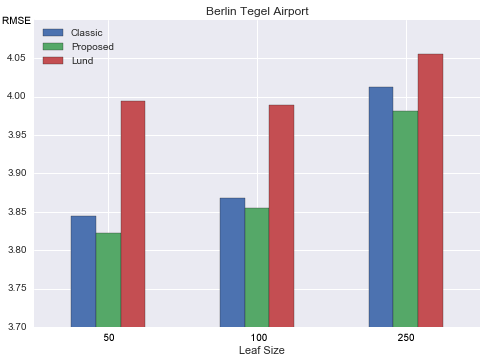
\includegraphics[width=8cm]{berlin.png}
  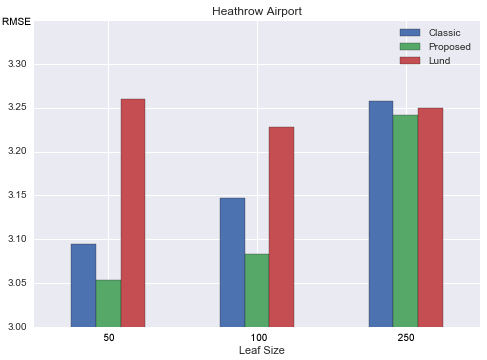
\includegraphics[width=8cm]{heathrow.png}
  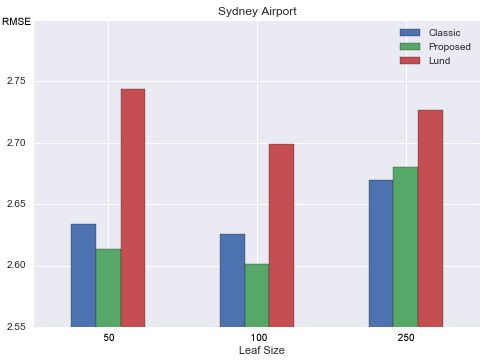
\includegraphics[width=8cm]{sydney.png}
  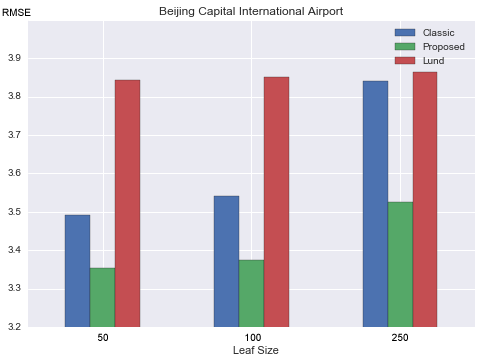
\includegraphics[width=8cm]{beijing.png}
  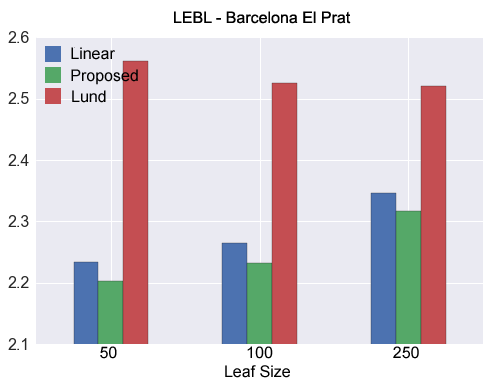
\includegraphics[width=8cm]{barcelona.png}
  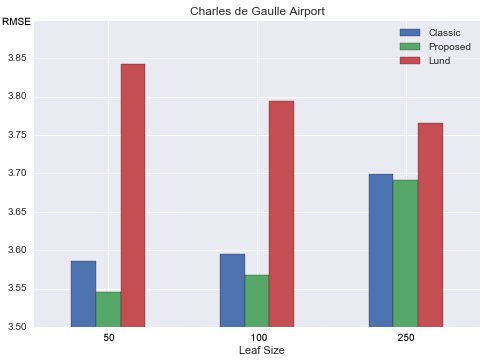
\includegraphics[width=8cm]{charles.png}
  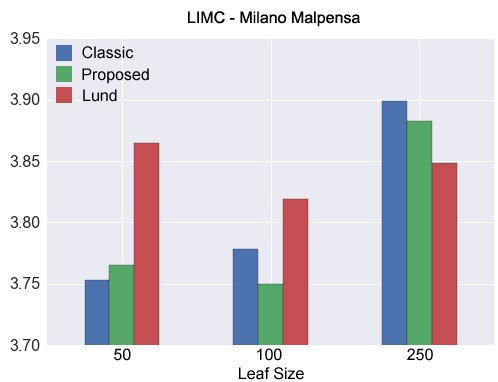
\includegraphics[width=8cm]{milan.png}
\caption{RMSE values for each airport comparing the accuracy of regression trees for different maximum leaf sizes.}
\label{f6}
\end{figure*}

The Nemenyi test pairwise compares every methodology. The performance of two methodologies is significantly different if the corresponding average rank differs by at least the critical difference. Figure \ref{f7} contains a representation of the results of the Nemenyi test comparing RMSE results for the three methodologies, one test per leaf size. These tests have been performed using the \textit{scmamp} R package publicly available at the Comprehensive R Archive Network (CRAN) \citep{Calvo2015}. Figure \ref{f7} represents the results of this test for a significance level $ p < 0.05 $ as CD diagrams.  These diagrams connect the groups of algorithms that are not significantly different, or in other words, whose distance is less than the critical difference, shown above the graph. As can be seen in the diagrams shown in Figure \ref{f7}, the proposed methodology outperforms the other two.

\begin{figure}
\centering
\parbox{5cm}{
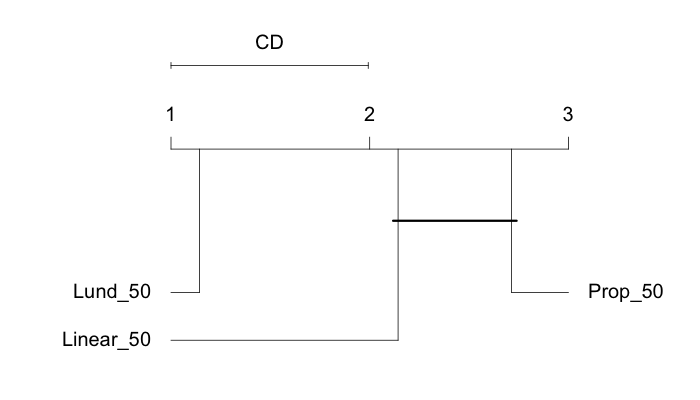
\includegraphics[width=5cm]{CD_50.png}}
\qquad
\begin{minipage}{5cm}
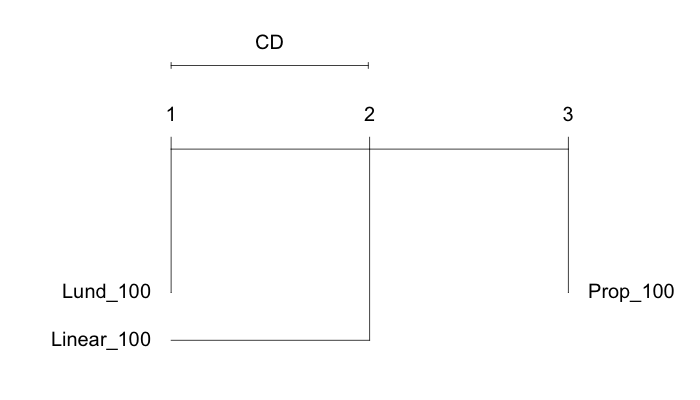
\includegraphics[width=5cm]{CD_100.png}
\qquad
\end{minipage}
\qquad
\begin{minipage}{5cm}
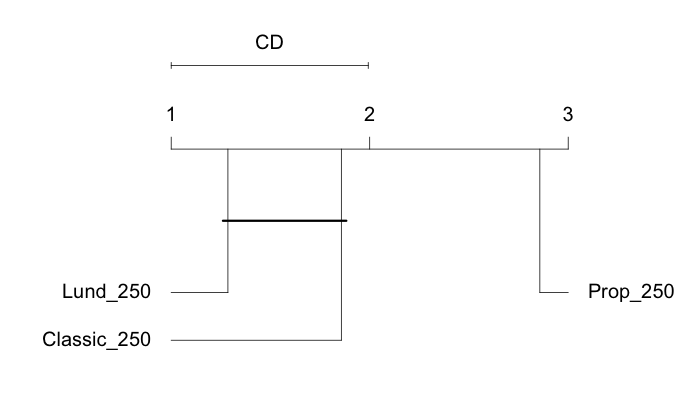
\includegraphics[width=5cm]{CD_250.png}
\qquad
\end{minipage}
\caption{Critical Difference figures comparing the three methodologies for the different leave sizes.}
\label{f7}
\end{figure}

One of the most significant aspects of these results is the different evolution, for each compared method, for the different maximum leaf sizes considered. For most of the airports, both the classic linear and the proposed methodologies improve their performance as the maximum leaf size is reduced. On the other hand, Lund's method presents no difference or degrades as the leaf size is reduced. This is a sign of poor generalisation of the splits lower down in the tree. Tests to detect the nature of this problem show that the error at training time also increases for this data set. This suggests that the use of non-contiguous splits for circular variables do not provide a good generalisation for subsequent splits performed by the tree.

\section{Conclusion and Future Work}
\label{sec:5}
This work revisits the idea of circular regression trees presenting a new methodology that improves the accuracy and performance of the previous proposal. Our proposal introduces the novelty of creating contiguous splits for the circular variables in a regression tree. Despite non contiguous splits are a more expressive way of partitioning a data set, they can suffer from bad generalisation. Regression trees are built using a recursive greedy methodology, where finding a local minimum in a node does not assure finding the best possible subsequent splits. Non-contiguous splits usually aggregate disjoint parts of a data set. The correlation between these parts might not generalise well for subsequent splits or new data.

This paper explores the fundamental differences in partitioning the space used by regression trees. Regression trees since they where first introduced have evolved with the introduction of many different techniques to improve their performance. Well known techniques such as pruning, balancing, smoothing \citep{Breimanetal1984, Quinlan1993} or ensembles \citep{Buhlmann2012} can remarkably improve the accuracy of the results when compared to basic regression trees.

Future work can introduce the ideas presented in this paper into more advanced implementations of regression trees. Creating contiguous splits in circular variables is an analogous process of the one followed in linear variables. Existing implementations of regression trees can be adapted to compute circular trees by introducing the mechanism of tagging circular variables and computing the first split by dividing the circular space into two bounded regions. Subsequent splits can be performed using the traditional methodology.

Each data set is different and normally it is a challenge to identify a methodology that performs well in every possible case. Non-contiguous splits can still be a good option and can better capture the relationships between different variables in some cases. This applies not only to circular variables but also to linear ones. An interesting line of further research could be to identify scenarios where non-contiguous splits have a benefit over contiguous ones.


\section*{Acknowledgements}

We would like to thank the Australian National Computational Infrastructure and the University of the Basque Country for their support and advice in carrying out this research work.
Our gratitude for the Basque Government program IT609- 13 and the Spanish Ministry of Economy and Competitiveness program TIN2013-41272P.


\bibliographystyle{model2-names}
\bibliography{refs}


\section*{Supplementary Material}

The implementation of the different versions of regression trees and the experiments are in Python language. The code has been made available using a public Git repository and can be accessed at:

\begin{verbatim}
 http://github.com/monkeybutter/circular_tree/
\end{verbatim}

This code contains the programs to run the experiments and produce the figures included in this work as well as an iPython notebook where some of the basic operations to train and test trees are explained.

Supplementary material that may be helpful in the review process should be prepared and provided as a separate electronic file. That file can then be transformed into PDF format and submitted along with the manuscript and graphic files to the appropriate editorial office.

\end{document}

%%
